\documentclass[12pt]{article}
\usepackage{amsmath}
\usepackage{fullpage}
\usepackage[authoryear,round]{natbib}
\usepackage{lineno}
\usepackage{graphicx} 
\usepackage{setspace}
\doublespacing
\sloppy

\title{Density-dependent selection and the limits of relative fitness}
\author{Jason Bertram $^{1,\ast}$ \\ 
Joanna Masel $^{1}$}

\date{}

\begin{document}

\maketitle

\noindent{}1. Department of Ecology and Evolutionary Biology, University of Arizona, Tucson, AZ 85721.

\noindent{}$\ast$ Corresponding author; e-mail: jbertram@email.arizona.edu.

\bigskip

\textit{Keywords}: Lottery model, competitive Lotka-Volterra, $r$/$K$-selection, interference competition, eco-evo.

\bigskip

\textit{Author contributions}: JB and JM conceptualized the manuscript. JB did the formal analysis. JB wrote the manuscript with review and editing from JM. 

\bigskip

\textit{Running title}: Density-dependence and relative fitness

\bigskip

\textit{Acknowledgments}: We thank Peter Chesson and Joachim Hermisson for many constructive comments on an earlier and quite different version of this manuscript. This work was financially supported by the National Science Foundation (DEB-1348262) and the John Templeton Foundation (60814).

\linenumbers{}
\modulolinenumbers[1]

\newpage{}


\section*{\centering \huge  Density-dependent selection and the limits of relative fitness}

\bigskip

\subsection*{Abstract}

Selection is commonly described in terms of relative fitness. Yet when selection is strong, the ecological view of selection in density-regulated populations seems to be incompatible with widely-used, constant-density relative fitness models such as the Wright-Fisher. Here we analyze the population ecological limits of relative fitness using a novel generalization of the Wright-Fisher model in which population density depends dynamically on the demographic rates of the types present. Our model contains a ``reproductive excess’’, and clearly distinguishes between density-dependent selection and selection-dependent density. These two effects are confounded in standard models of density-regulated population growth. Both effects are necessary, in combination with strong selection, for relative fitness to break down in populations close to demographic equilibrium. Remarkably, both effects are not sufficient: we give an example of strong selection on a density-regulating trait subject to density-dependent selection that conforms to the relative fitness description almost exactly. We reiterate the importance of reproductive excesses in many species, which allows even strong selection to have no effect on density. Our model also offers a possible alternative to relative fitness when the latter is untenable, as is likely the case far from demographic equilibrium. 

\noindent (191 words)



\newpage{}


\section*{Introduction}

There are a variety of different measures of fitness. Some widely used examples are expected lifetime reproductive ratio $R_0$, intrinsic population growth rate $r$, saturation population density/carrying capacity (often labeled ``$K$'') \citep{benton_2000}, and invasion fitness \citep{metz_1992}. In addition, ``relative fitness'' is the standard in much of evolutionary biology, particularly evolutionary genetics, where the focus is relative genotypic proportions \cite[pp. 468]{barton_2007}. The variety of fitness measures is not problematic in itself, because different measures have different uses. But it should be clear how these measures are connected to the processes of birth and death which ultimately drive selection \citep{metcalf_2007,doebeli_2017}. While such a connection is fairly clear for absolute fitness measures like $r$, relative fitness is largely divorced from population ecology. It has even been proposed that relative fitness be justified from measure theory, abandoning population biology altogether \citep{wagner_2010}. Given the ubiquitous use of relative fitness, it is important that we understand its population ecological basis, both to clarify its domain of applicability, and as part of the broader challenge of synthesizing ecology and evolution.

Constant relative fitness values can be justified as an approximation which holds when selection is sufficiently weak and stable over time. Formally, these values are the ``zeroth order'' components of the actual relative fitnesses, which are not constant but depend on density, frequency, age structure, and so on \cite[pp. 277]{ewens_2004} \citep[Chap. 4]{charlesworth_1994}. Yet strong, temporally-variable selection occurs widely in nature and the lab, including in wild \textit{Drosophila}, where population density also varies by orders of magnitude each seasonal cycle \citep{messer_2016,bergland_14}. The question is whether relative fitness can be used when selection is not vanishingly weak. In general, age-structured populations that reproduce by outcrossing do not permit strong selection to be represented in terms of type-specific relative-fitness constants \citep[Chap. 4]{charlesworth_1994}. We will therefore restrict our attention to asexual haploids with little or no age structure, where it is easier to evaluate how the success or failure of the relative fitness description is tied to the underlying population ecological assumptions. 

In the absence of crowding, relative fitness simply represents differences in intrinsic population growth rate. In discrete time, the change in frequency of type $i$ is $\Delta p_i=\left(\frac{W_i}{\overline{W}}-1\right) p_i$, where $W_i$ is the intrinsic absolute growth factor of type $i$, and $\overline{W}=\sum_i W_i p_i$ is the population mean $W$. The change in frequency depends only the relative ratio $\frac{W_i}{\overline{W}}$, not the absolute values of the growth factors $W_i$. Thus, we can replace the $W_i$ with any set of values $w_i$ that are proportional to the $W_i$; these values are called ``relative fitnesses''. The analogous formula in continuous time is $\frac{d p_i}{dt}=(r_i-\overline{r}) p_i$, where $W_i$ is replaced by the intrinsic exponential growth rate $r_i$ \citep[pp. 26]{crow_1970}, and the ratio $\frac{W_i}{\overline{W}}$ is replaced by the difference $r_i-\overline{r}$. In the particular case that there are two types present, a wildtype $i$ and a mutant $j$ for instance, then the continuous time equation takes the familiar form
\begin{equation}
\frac{d p_i}{dt}=s p_i(1-p_i), \label{eq:canonical}
\end{equation}
where $s=r_i-r_j$ is the selection coefficient. 

The simple interpretation of relative fitness as a difference in intrinsic growth rates breaks down when we allow for population crowding. Since crowded and uncrowded conditions are so different, we expect that $s$ will often depend on density \citep{travis_2013}. Eq.~\eqref{eq:canonical} is then no longer a complete description of selection --- we would also need to specify a model for how density is changing. Note that frequency-dependent selection does not raise similar problems; Eq.~\eqref{eq:canonical} is still a complete description of selection even if its behavior is more complicated due to $s$ depending on frequency. Population genetics traditionally evades the issue of density-dependent selection by simply assuming that total population density $N$ has reached its equilibrium value, which is assumed to be a fixed constant. The selection coefficient $s$ now abstractly parameterizes the rate at which selection changes relative frequencies, and no longer corresponds to differences in intrinsic growth rates $r$. 

However, MacArthur famously argued that when population growth is density-regulated, selection in crowded populations is intimately connected to the ability to keep growing at higher densities than other types can tolerate \citep{macarthur_1967}. The classic example is the logistic model, where the type with the greatest saturation population density ``$K$'' excludes the others (Fig.~\ref{fig:Ksel}a). Similarly, the ``$R^*$ rule'', a central tenet of resource competition theory, states that when growth is limited by a single homogeneous consumable resource, the type able to deplete the resource to the lowest equilibrium density $R^*$ excludes the others \citep{grover_1997}. Differences in $R^*$ will often entail differences in saturation density. The Lotka-Volterra competition model also couples selection in crowded populations to density except in special cases \citep{smouse_1976,mallet_2012}. In these examples, both $N$ and $s$ change during, and as a result of, adaptive sweeps. It would therefore seem that the ubiquitous constant-$N$, relative fitness description of selection is incompatible with a huge class of population ecological processes driving selection (Fig.~\ref{fig:Ksel}b), even in the absence of age-structure and mating.

\begin{figure}
\centering
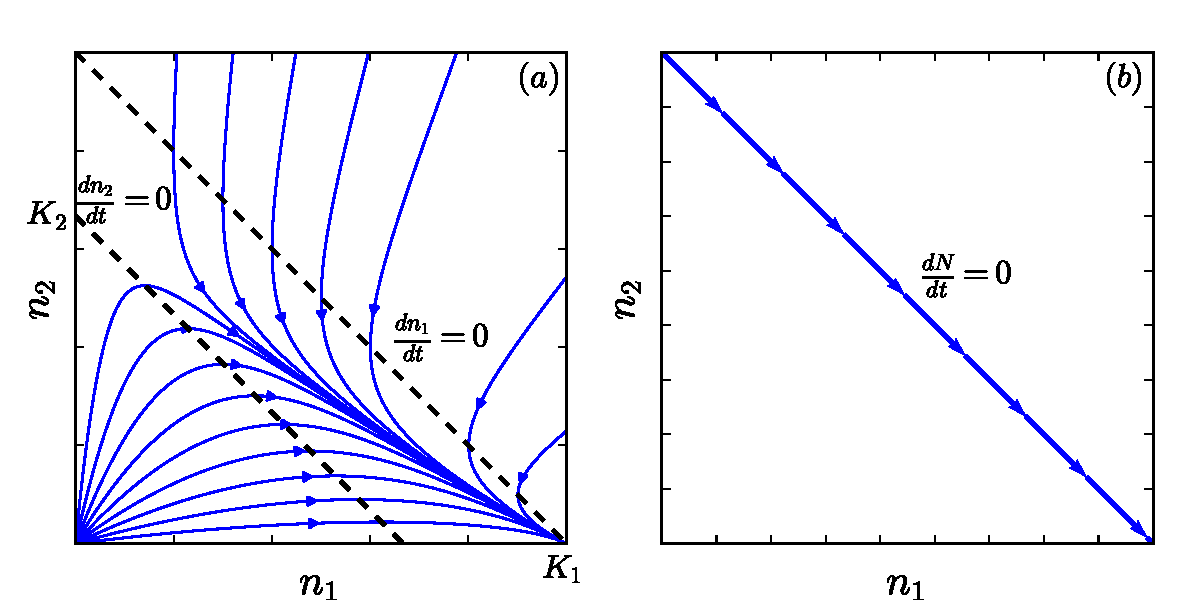
\includegraphics[scale=0.8]{Kplot.pdf}
\caption{\label{fig:Ksel} Selection in crowded environments shown as a phase diagram for the densities of two types $n_1$ and $n_2$. (a) The logistic model $\frac{dn_1}{dt}=r_1(1-\frac{n_1+n_2}{K_1})n_1$ and $\frac{dn_2}{dt}=r_2(1-\frac{n_1+n_2}{K_2})n_1$ with $r_1=r_2$ and $K_1>K_2$. (b) The constant-$N$, relative fitness description of selection.}
\end{figure}

In light of this difficulty, the relative fitness description has been justified in broadly two different ways for crowded populations (we do not discuss Wagner's [\citeyear{wagner_2010}] measure-theoretical justification, which is independent of population biology). The first is to simply assume that selection is density-independent but relax the assumption of constant $N$ by allowing density to change as a result of selective sweeps \citep[pp. 468]{barton_2007} \citep{prout_1980}. Obviously this does not address the problem that $s$ can, in reality, depend on density. Type-specific responses to density are at the center of MacArthur's argument and the density-dependent selection literature that grew out of it (e.g. \citep{roughgarden_1979}). 

The second justification, which primarily grew out of a controversy over Haldane's ``cost of selection'', is to appeal to the existence of a ``reproductive excess'' of juveniles that are more fragile than their adult counterparts \citep{turner1968population,kimura1969natural,nei1971fertility}. Selection can then be concentrated at the juvenile phase, uncoupling selection from population density at the adult phase unless it is so strong that the reproductive excess is depleted. This justifies Eq.~\eqref{eq:canonical} because, for a population in demographic equilibrium, selective sweeps do not affect density, and so the density-dependence of selection does not matter. Unfortunately this reproductive excess literature is also poorly integrated with population ecology. \cite{kimura1969natural} took constant $N$ as a requirement and then derived some variants of the logistic model that satisfy this requirement. \cite{nei1971fertility} proposed a model with an explicit representation of reproductive excess, but used an unusual model of competition based on pair-wise interactions which was only defined for at most two different types. As a result, the role of reproductive excesses in justifying Eq.~\eqref{eq:canonical} is still largely verbal.

Here we study the population ecology of relative fitness using a novel model of density-dependent population growth based on territorial contests. Rather than attempting to make sense of relative fitness in existing standard models of population growth (e.g. \citep{kimura1969natural,mallet_2012}), we instead do the reverse, and attempt to make population ecological sense of the widely-used Wright-Fisher relative-fitness model. 

Our starting point is the classic lottery model of territorial contest \citep{sale_77,chesson_1981}. The classic lottery assumes a saturated population with constant $N$, and fitness involves a product of fertility and juvenile viability \citep[pp. 185]{crow_1970}, but unlike the Wright-Fisher model, generations can overlap. 

Our first task is to generalize the lottery model to create a variable-density version of the Wright-Fisher model with overlapping generations (sections ``Model'' and ``Analytical approximation of the variable-density lottery''). 

Equipped with this new model, we turn to the evaluation of Eq.~\eqref{eq:canonical}. We first discuss selection on the ability to contest territories, which behaves like a pure constant-$N$, relative fitness trait, and discuss how this fits with MacArthur's analysis of selection in crowded populations (section ``$K$-selection and selection-dependent density''). We then consider selection on density-regulating traits (section ``Density-regulating traits and the threat of strong selection''), and conclude by contrasting the classical density-dependent selection literature with our results (``Discussion'').
 
\section*{Model}\label{sec:model}

\subsection*{Assumptions and definitions} 

We assume that reproductively mature individuals (``adults'') require their own territory to survive and reproduce. All territories are identical, and the total number of territories is $T$. Time advances in discrete iterations, each representing the time from birth to reproductive maturity. In a given iteration, the number of adults of the $i$'th type will be denoted by $n_i$, the total number of adults by $N=\sum_i n_i$, and the number of unoccupied territories by $U=T-N$. We assume that the $n_i$ are large enough that stochastic fluctuations in the $n_i$ (``drift'') can be ignored (with $T$ also assumed large to allow for low type densities $n_i/T$).

\begin{figure}
\centering
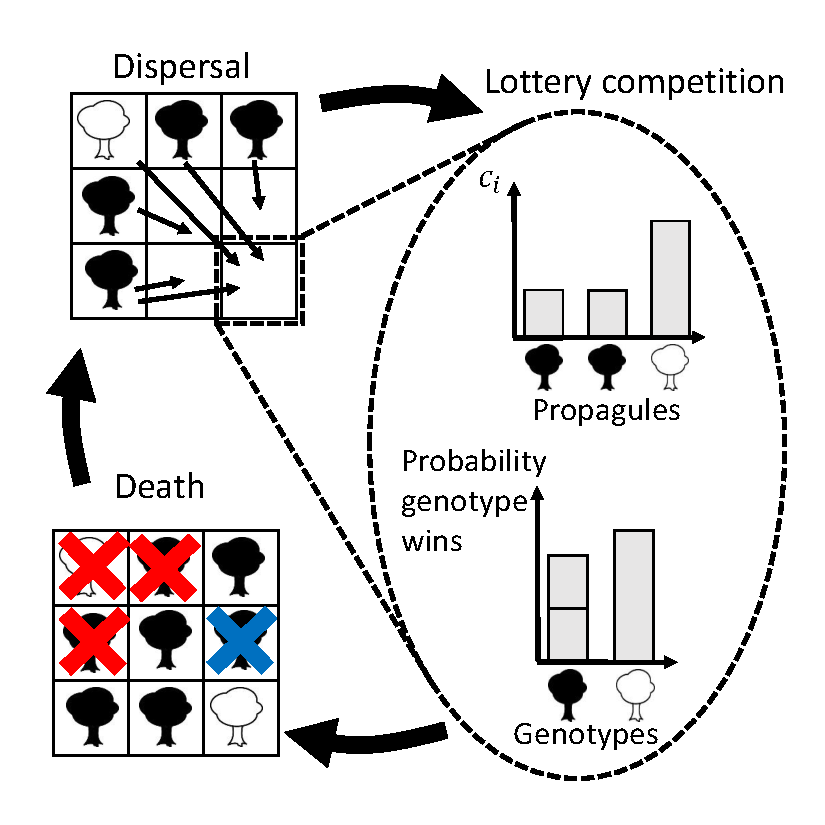
\includegraphics[scale=0.8]{lottery.pdf}
\caption{\label{fig:lottery} One iteration of our model. Propagules are dispersed by adults at random (only propagules landing on unoccupied territories are shown). Territories can receive zero propagules. Lottery competition then occurs in each territory that receives more than one propagule (only illustrated in one territory). In a given territory, each type has probability proportional to $c_i x_i$ of winning the territory, where $c_i$ measures competitive ability and $x_i$ is the number of $i$ propagules present. In the illustrated territory, more black propagules are present, but white is a stronger competitor and has a higher probability of winning. Territories are made available for the next iteration by the death of adults present at the start of the iteration (red crosses).}
\end{figure}

Each iteration, adults produce propagules which disperse at random, independently of distance from their parents, and independently of each other. We assume that each adult from type $i$ produces $b_i$ propagules on average, so that the mean number of $i$ propagules dispersing to unoccupied territories is $m_i=b_in_iU/T$. The parameter $b_i$ can be thought of as a measure of ``colonization ability'', which combines fecundity and dispersal ability \citep{levins_71,tilman_94,bolker_99}. Random dispersal is then modeled using a Poisson distribution $p_i(x_i)=l_i^{x_i} e^{-l_i}/x_i!$ for the number $x_i$ of $i$ propagules dispersing to any particular unoccupied territory, where $l_i=m_i/U$ is the mean propagule density in unoccupied territories. The total propagule density will be denoted $L=\sum_i l_i$.

We assume that adults cannot be ousted by juveniles, so that recruitment to adulthood occurs exclusively in unoccupied territories. When multiple propagules land on the same unoccupied territory, the winner is determined by lottery competition: type $i$ wins a territory with probability $c_i x_i/\sum_i c_i x_i$, where $c_i$ is a constant representing relative competitive ability (Fig. \ref{fig:lottery}). Since the expected fraction of unoccupied territories with propagule composition $x_1,\ldots,x_G$ is $p_1(x_1)\cdots p_G(x_G)$ where $G$ is the number of types present, and type $i$ is expected to win a proportion $c_i x_i/\sum_i c_i x_i$ of these, type $i$'s expected territorial acquisition is given by
\begin{equation}
\Delta_+ n_i=U\sum_{x_1,\ldots,x_G} \frac{c_i x_i}{\sum_i c_i x_i} p_1(x_1)\cdots p_G(x_G). \label{eq:growthsumuncoupled}
\end{equation}
Here the sum only includes territories with at least one propagule present. Since we do not consider drift here, we will not analyze the fluctuations around these two expectations.

Adult mortality only occurs in adults present at the start of the  iteration, and at a constant, type-specific per-capita rate $0\leq d_i\leq 1$ (Fig.~\ref{fig:lottery}). This gives an overall change in type abundances of
\begin{equation}
\Delta n_i=\Delta_+ n_i-d_i n_i. \label{eq:delttot}
\end{equation}

\subsection*{Connection to the classic lottery model}

In the classic lottery model \citep{chesson_1981}, unoccupied territories are assumed to be saturated with propagules from every type ($l_i\rightarrow \infty$ for all $i$). From the law of large numbers, the composition of propagules in each territory will not deviate appreciably from the mean composition $l_1,l_2,\ldots,l_G$. Type $i$ is thus expected to win a proportion $c_i l_i/\sum_i c_i l_i$ of the $U$ available territories,
\begin{equation}
\Delta_+ n_i=\frac{c_i l_i}{\sum_i c_i l_i}U=\frac{c_i l_i}{\overline{c}L}U, \label{eq:lottery}
\end{equation}
where $\overline{c}=\sum_i c_i m_i/\sum_i m_i$ is the mean competitive ability for a randomly selected propagule. Note that all unoccupied territories are filled in a single iteration of the classic lottery model, whereas our more general model Eq.~\eqref{eq:growthsumuncoupled} allows for territories to be left unoccupied and hence also accommodates low propagule densities.

\section*{Results}

\subsection*{Analytical approximation of the variable-density lottery}

Eq.~\eqref{eq:growthsumuncoupled} involves an expectation over the time-dependent dispersal distributions $p_i$. Here we evaluate this expectation to obtain a better intuition about the dynamics of density-dependent lottery competition. 

Similarly to the high-$l_i$ approximation of the classic lottery model, we replace the $x_i$ in Eq.~\eqref{eq:growthsumuncoupled} with ``effective'' mean values, although we cannot simply use the means $l_i$ as in the classic lottery. For a rare type, growth comes almost entirely from territories with $x_i=1$, for which its mean density $l_i\ll 1$ is not representative. We therefore separate Eq.~\eqref{eq:growthsumuncoupled} into $x_i=1$ and $x_i>1$ components. Our more general approximation only requires that there are no large discrepancies in competitive ability (i.e. we do not have $c_i/c_j\gg 1$ for any two types). We obtain (details in Appendix B)
\begin{equation}
\Delta_+ n_i\approx \left[e^{-L}+(R_i+A_i)\frac{c_i}{\overline{c}}\right]l_i U, \label{eq:master}
\end{equation}
where
\begin{equation}
R_i=\frac{\overline{c}e^{-l_i}(1-e^{-(L-l_i)})}{c_i +\frac{\overline{c}L- c_il_i}{L-l_i}\frac{L-1+e^{-L}}{1-(1+L)e^{-L}}},\nonumber \label{eq:Dr}
\end{equation}
and
\begin{equation}
A_i=\frac{\overline{c}(1-e^{-l_i})}{\frac{1-e^{-l_i}}{1-(1+l_i)e^{-l_i}}c_il_i+\frac{\overline{c}L- c_il_i}{L-l_i}\left(L\frac{1-e^{-L}}{1-(1+L)e^{-L}}-l_i\frac{1-e^{-l_i}}{1-(1+l_i)e^{-l_i}}\right)}. \nonumber \label{eq:Da}
\end{equation}

Comparing Eq. \eqref{eq:master} to Eq. \eqref{eq:lottery}, the classic lottery per-propagule success rate $c_i/\overline{c}L$ has been replaced by three separate terms. The first, $e^{-L}$, accounts for propagules which land alone on unoccupied territories; these propagules secure the territories without contest. The second, $R_i c_i/\overline{c}$, represents competitive victories on territories where only a single $i$ propagule lands, and at least one other propagule from a different type (this term dominates the growth of a rare invader in a high density population and determines invasion fitness). The third term, $A_i c_i/\overline{c}$, represents competitive victories in territories where two or more $i$ type propagules are present. The relative importance of these three terms varies with both the overall propagule density $L$ and the relative propagule frequencies $l_i/L$. If $l_i\gg 1$ for all types, we recover the classic lottery model (only the $A_ic_i/\overline{c}$ term remains, and $A_i\rightarrow 1/L$). 

Fig.~\ref{fig:simcomp} shows that Eq. \eqref{eq:master} and its components closely approximate simulations of our variable-density lottery model over a wide range of propagule densities.  Two types are present, one of which is at low frequency. The growth of the low-frequency type relies crucially on the low-density competition term $R_i c_i/\overline{c}$. On the other hand, $R_i c_i/\overline{c}$ is negligible for the high-frequency type, which depends instead on high density territorial victories. Fig.~\ref{fig:simcomp} also shows the breakdown of the classic lottery model at low propagule densities.

\begin{figure}
\centering
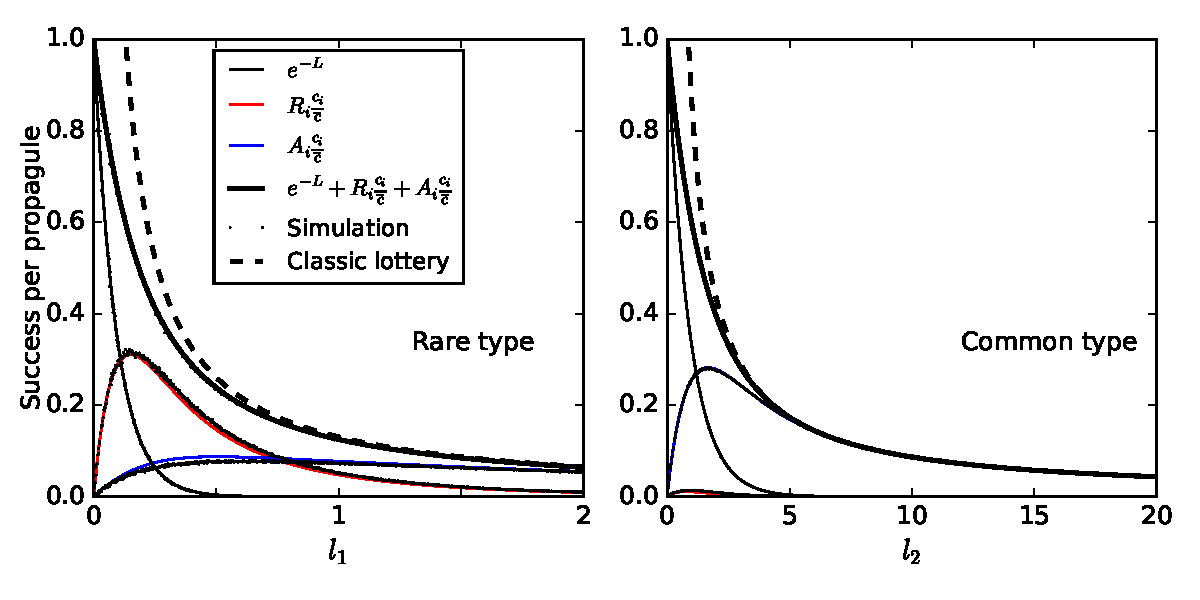
\includegraphics[scale=0.8]{simulationcomparison.pdf}
\caption{\label{fig:simcomp} Comparison of Eq.~\eqref{eq:master}, the classic lottery model, and simulations. The vertical axis is per-propagule success rate for all propagules $\Delta_+ n_i/m_i$, and for the three separate components in Eq.~\eqref{eq:master}. Simulations are 	conducted as follows: $x_1,\ldots,x_G$ values are sampled $U$ times from Poisson distributions with respective means $l_1,\ldots,l_G$, and the victor in each territory is then decided by random sampling weighted by the lottery win probabilities $c_ix_i/\sum_j c_j x_j$. Two types are present, a rare type with $c_1=1.5$, and a common type with $c_2=1$. Simulation points are almost invisible for the common type due to near exact agreement with Eq.~\eqref{eq:master}. Dashed lines show the breakdown of the classic lottery model. Parameters: $U=10^5$ and $l_1/l_2=0.1$ is kept fixed while varying the total density $L$.} 
\end{figure}

In the special case that all types are competitively equivalent (identical $c_i$), Eq.~\eqref{eq:master} takes a simpler form,
\begin{equation}
\Delta_+ n_i = \frac{l_i}{L}(1-e^{-L})U. \label{eq:masterequalc}
\end{equation}
This formula can also be deduced directly from Eq.~\eqref{eq:growthsumuncoupled}: $1-e^{-L}$ is the fraction of territories that receive at least one propagule under Poisson dispersal, $(1-e^{-L})U$ is the total number of such territories, and type $i$ is expected to receive a fraction $l_i/L$ of these. Total population density thus grows according to
\begin{equation}
\Delta N=(1-e^{-L})U-\sum_i d_i n_i \label{eq:Nmaster}
\end{equation}

\subsection*{Selection in the variable-density lottery}

We now outline the properties of selection in the variable-density lottery, starting with selection on competitive ability $c$. Eq.~\eqref{eq:Nmaster} shows that $c$ is not a density-regulating trait: $c$ only affects the relative likelihood for each type to win a contested territory, not whether a territory is contested in the first place. Selection between types which only differ in $c$ occurs without changing density $N$. However, $c$-selection is density-dependent, with the strength of selection (measured by the difference between types in the per-capita growth rate $\Delta n_i/n_i$) peaking at an intermediate density (Fig.~\ref{fig:DDS_lottery}). This intermediate peak occurs because most territories are claimed without contest at low density, whereas few unoccupied territories are available to be contested at high density. 

Turning to selection on the density-regulating traits $b$ and $d$, we write Eq.~\eqref{eq:masterequalc} in the form
\begin{equation}
\frac{\Delta n_i}{n_i} = \frac{b_i}{\overline{b}}\frac{1-e^{-\overline{b}N/T}}{N}(T-N)-d_i, \label{eq:bdensitydependence}
\end{equation}
where we have used that fact that $L=\overline{b}N/T$, and $\overline{b}$ is the population mean $b$. It is clear from Eq.~\eqref{eq:bdensitydependence} that selection on adult mortality $d$ is independent of density. On the other hand, $b$-selection is density-dependent. The advantage of having greater $b$ declines with density because fewer territories are available to to be claimed (Fig.~\ref{fig:DDS_lottery}). 

\begin{figure}
\centering
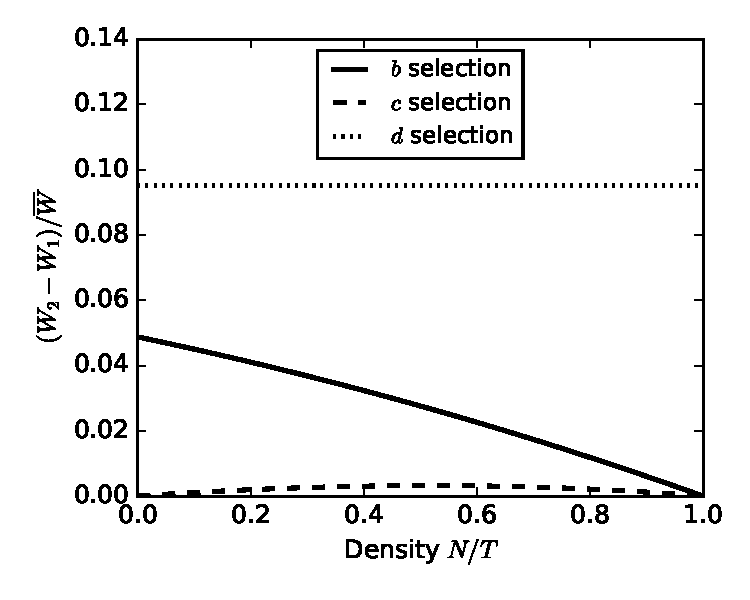
\includegraphics[scale=0.8]{DDS_lottery.pdf}
\caption{\label{fig:DDS_lottery} The density-dependence of selection in our variable-density lottery plotted as difference in propagule success rate $\Delta n_j/m_j-\Delta n_i/n_i$ between an adaptive variant $j$ and a wildtype $i$ present at the same frequency. Here $b_i=1$, $d_i=0.5$ and $c_i=1$. For $b$-selection we set $b_j=b_i(1+\epsilon)$, and similarly for $c$ and $d$, with $\epsilon=0.1$. $d$-selection is density-independent, $b$-selection gets weaker with lower territorial availability, while $c$-selection initially increases with density as territorial contests become more important, but eventually also declines as  available territories become scarce. The equilibrium density for the $i$ type is $\approx 0.4$.}
\end{figure}

\subsection*{Selection-dependent density and $K$-selection}

We now start evaluating the limits of Eq.~\eqref{eq:canonical} in the context of the variable-density lottery model, focusing in this section on the issue of whether density varies as a result of selection \citep{prout_1980}. We showed in the previous section that $c$-selection in the variable-density lottery does not affect density. 
However, this is not the case in most previous models of density-dependent selection, which have been strongly influenced by the notion of ``$K$-selection'' and the associated questions about whether selection in crowded populations will tend to increase population density \citep{anderson_1971,roughgarden_1979,lande_2009}. To clarify the connection between ``$K$-selection'' and the variable density lottery model, we thus revisit MacArthur's analysis of selection in crowded populations \citep{macarthur_1967}.

MacArthur considers a population with two types that have densities $n_1$ and $n_2$ subject to density-dependent growth described by
\begin{equation}
\frac{d n_1}{d t}=f_1(n_1,n_2)\qquad\frac{d n_2}{d t}=f_2(n_1,n_2). \label{eq:macgeneral}
\end{equation}
The environment is assumed to remain constant apart from the type densities. The functions $f_1$ and $f_2$ must decline to zero if $n_1$ or $n_2$ are sufficiently large, because no population has unlimited resources. This defines nullclines $f_1(n_1,n_2)=0$ and $f_2(n_1,n_2)=0$ in $(n_1,n_2)$ space. The outcome of selection is then determined by the relationship between these nullclines. Specifically, a type will be excluded if its nullcline is completely contained in the region bounded by the other type's nullcline. In other words, for a type to have the possibility of persisting, it must be able to keep growing to higher densities than the other type can tolerate in some region of $(n_1,n_2)$ space (Fig.~\ref{fig:Ksel}a).

To formalize the relationship between nullclines, MacArthur used the symbol ``$K$'' to label the four intersection points of the nullclines with the $n_1$ and $n_2$ axes, specifically $f_1(K_{11},0)=0$, $f_1(0,K_{12})=0$, $f_2(0,K_{22})=0$ and $f_2(K_{21},0)=0$. These $K$ values determine whether a region of higher-density growth exists for each type, provided that the nullclines are close to being straight lines. Note that only $K_{11}$ and $K_{22}$ are saturation densities akin to the $K$ parameter in the logistic model; following widespread convention, we will refer to selection on these saturation densities as ``$K$-selection'' (Fig.~\ref{fig:Ksel}a). The other intersection points, $K_{12}$ and $K_{21}$, are related to competition between types. For instance, in the Lotka-Volterra competition model we have
\begin{align}
f_1(n_1,n_2) = r_1(1-\alpha_{11}n_1-\alpha_{12}n_2)n_1\nonumber\\
f_2(n_1,n_2) = r_2(1-\alpha_{22}n_1-\alpha_{21}n_2)n_2\label{eq:LV}
\end{align}
where $\alpha_{11}=1/K_{11}$ and $\alpha_{22}=1/K_{22}$ measure competitive effects within types, while $\alpha_{12}=1/K_{12}$ and $\alpha_{21}=1/K_{21}$ measure competitive effects between types (Fig.~\ref{fig:LVvslottery}a). 

In summary, MacArthur's conclusion that  ``fitness is $K$'' in crowded populations \citep[pp. 149]{macarthur_1967} means that selection either favors the ability to keep growing at ever higher densities (moving a type's own nullcline outwards), or the ability to suppress the growth of competitors at lower densities (moving the nullcline of competitors inwards) \citep{gill_1974}. This general idea is much broader than ``$K$-selection'' in the sense of selection for greater saturation density, and applies even if the nullclines are nonlinear to such an extent that the ``$K$'' values themselves do not give much information about the regions of high-density growth.

\begin{figure}
\centering
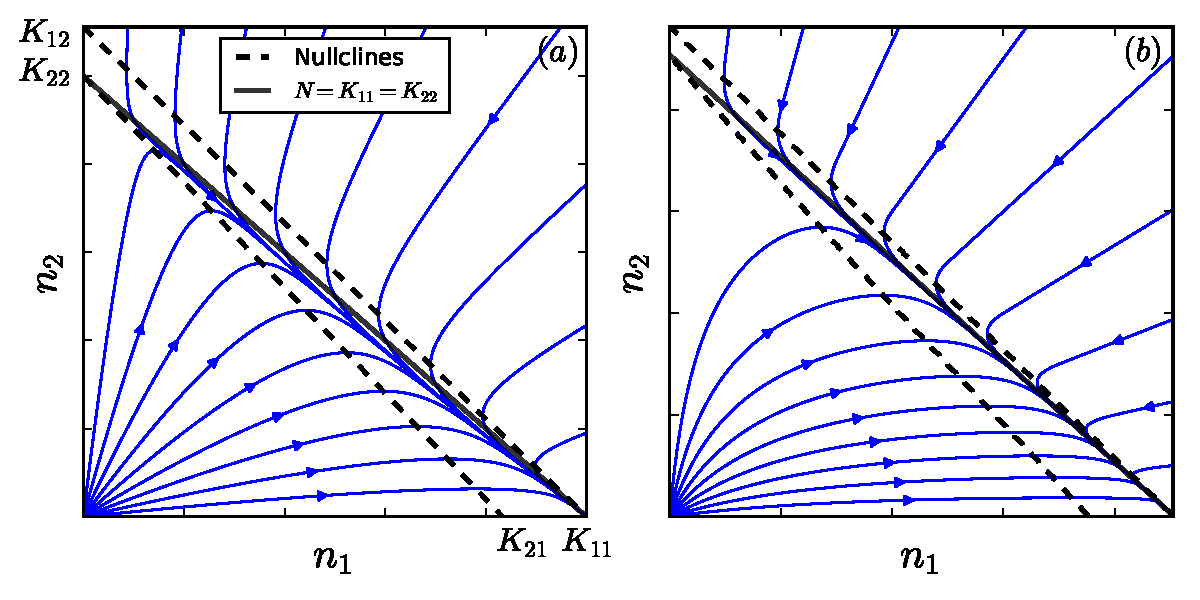
\includegraphics[scale=0.8]{LVvslottery.pdf}
\caption{\label{fig:LVvslottery} Selection between types with identical saturation density but different inter-type competitive ability. (a) Lotka-Volterra competition (Eq.~\ref{eq:LV}) with $r_1=r_2=1$, $\alpha_{11}=\alpha_{22}=1$, $\alpha_{12}=0.9$ and $\alpha_{21}=1.2$. Trajectories do not follow the line $N=K_{11}=K_{22}$. (b) Lottery competition (Eq.~\ref{eq:master}) with $b_1=b_2=5$, $d_1=d_2=0.1$ and $c_1/c_2=5$. Trajectories converge on the line $N=K_{11}=K_{22}$.}
\end{figure}

It is obvious in the Lotka-Volterra model that selection can favor a superior competitor in a crowded population even if its saturation density is lower than that of the other types present. Nevertheless, the Lotka-Volterra model still couples population density to selection \citep{smouse_1976}. Fig.~\ref{fig:LVvslottery}a shows Lotka-Volterra selection between two types with the same saturation density ($\alpha_{11}=\alpha_{22}$, $\alpha_{21}>\alpha_{12}$). Even though the initial and final densities of a sweep are the same, density is not constant over a sweep (constant density is possible but only occurs for a highly restricted subset of $r$ and $\alpha$ values; further details in Appendix C; also see \citealt{mallet_2012}). Intuitively, for one type to exclude another with the same saturation density, competitive suppression of growth between types must be stronger than competitive suppression of growth within types, causing a dip in $N$ over the sweep. 

By contrast, density trajectories in the variable-density lottery model converge on the saturation density line (Fig.~\ref{fig:LVvslottery}b). Selection then occurs along this line, similarly to Fig.~\ref{fig:Ksel}b. In other words, once the population reaches demographic equilibrium, it behaves indistinguishably from a constant-$N$ relative fitness model. This behavior occurs because $c$ determines relative competitive success in territorial contests. As such, it is a manifestation of a reproductive excess of propagules. Previous models of selection-independent density have either relied on unusual models of competition \citep{kimura1969natural,nei1971fertility}, or made restrictive Lotka-Volterra parameter choices (Appendix C; \citealt{smouse_1976,mallet_2012}).

\subsection*{Density-regulating traits and the threat of strong selection}

In the previous section we showed that $c$-selection and the regulation of population density are independent even though population growth is density-regulated in our variable-density lottery. Nevertheless, selection and density regulation \textit{are} intimately connected in widely used models of population growth, as well as for the lottery $b$ and $d$ traits.

To see why this connection potentially poses a threat to relative fitness, consider the simple birth-death model \cite[pp. 20]{kostitzin_1939} \citep{travis_2013} 
\begin{equation}
\frac{d n_i}{dt}=(b_i -\delta_iN) n_i \label{eq:simplebirthdeath}
\end{equation}
where $\delta_i$ is the per-capita increase in mortality rate due to crowding (for simplicity, there are no deaths when uncrowded), playing a similar role as $1/K$ in the logistic model. 

Starting from a monomorphic population, the frequency of a variant with $\delta_j=\delta_i(1-\epsilon)$ obeys 
\begin{equation}
\frac{d p_j}{dt}=\epsilon \delta_i N p_j(1-p_j). \label{eq:Ndependentsweep}
\end{equation}
The selection coefficient $s=\epsilon \delta_i N$ thus depends on density (compare with Model III in \cite{kimura1969natural}). On the other hand, the frequency of a variant with $b_j= b_i(1+\epsilon)$ will exactly obey Eq.~\eqref{eq:canonical} with $s=\epsilon b_i$, independent of density.

In practice the density dependence in Eq.~\eqref{eq:Ndependentsweep} only matters if $N$ changes substantially during a sweep. This can easily occur if a population is far from demographic equilibrium (we return to this scenario in the Discussion). However, even if $N$ has reached equilibrium, it will change substantially over a $\delta$-sweep if selection on $\delta$ is sufficiently strong. To quantify this effect, we need to account for how much $N$ changes as a result of a $\delta$-sweep beginning and ending in equilibrium \citep{kimura1969natural}; from Eq.~\eqref{eq:simplebirthdeath} we have an increase from $N_{\rm initial}=b_i/\delta_i$ to $N_{\rm final}=b_i/(\delta_i(1-\epsilon))=N_{\rm initial}/(1-\epsilon)$. The corresponding selection coefficient increases from $s_{\rm initial}= \epsilon b_i$ to $s_{\rm final}=s_{\rm initial}/(1-\epsilon)$. Consequently, noticeable deviations from Eq.~\eqref{eq:canonical} occur with proportional changes to $\delta$ of order $\epsilon=0.2$ and upwards i.e. selection must be quite strong (Fig.~\ref{fig:strengthofselection}). 

\begin{figure}
\centering
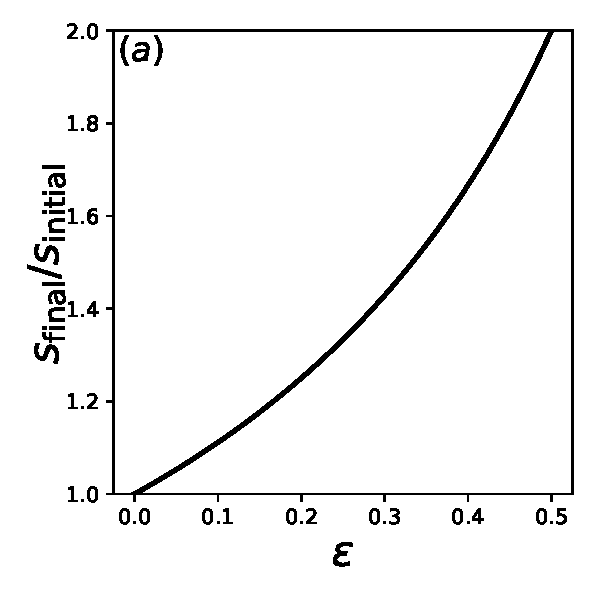
\includegraphics[scale=0.8]{strengthofselection.pdf}
\caption{\label{fig:strengthofselection} (a) Proportional change in the selection coefficient over a ``$K$-like'' sweep for a type that experiences proportionally $1-\epsilon$ fewer deaths induced by crowding. The population is in demographic equilibrium at the start and end of the sweep. (b) Example equilibrium-to-equilibrium $\delta$-sweep (Eq.~\ref{eq:Ndependentsweep}) for $\epsilon=0.2$ showing a noticeable deviation from the canonical selection equation.}
\end{figure}


 Thus, $d$ sweeps follow the canonical relative fitness model exactly (Fig.~\ref{fig:DDS_lottery}).
 
 At first glance, $b$ in Eq.~\eqref{eq:bdensitydependence} appears to be analogous to the $\delta$ in Eq.~\eqref{eq:simplebirthdeath} because it regulates density and is multiplied by the density-dependent term $f(\overline{b},N)=\frac{1-e^{-\overline{b}N/T}}{N}(T-N)$. 


Nevertheless, the behavior of equilibrium-to-equilibrium $b$-sweeps are qualitatively different from the $\delta$ sweeps above. The reason is that $b$ regulates density by controlling how many unoccupied territories receive propagules. Thus, greater $b$ means more propagules contesting territories, but also more territories being contested. The net effect on $f(\overline{b},N)$ is precisely zero in equilibrium: in a single-type equilibrium we have $b_i/\overline{b}=1$ and so $f(\overline{b},N)=d_i$ exactly at the beginning and end of a pure $b$ sweep, even though the density $N$ increases. Strictly speaking there is some deviation in $f(\overline{b},N)$ from $d_i$ during the sweep, but this deviation is an order of magnitude smaller than for a $\delta$ sweep (the deviation due to a sweep with proportional effect $b_j= b_i(1+\epsilon)$ is only of order $\epsilon^2$, whereas the analogous effect in Fig.~\ref{fig:strengthofselection} is of order $\epsilon$; see Appendix D for details). Since selection must already be quite strong for a $\delta$ sweep to threaten Eq.~\eqref{eq:canonical}, we conclude that $b$ sweeps also obey the canonical selection equation (to a close approximation). 

\section*{Discussion}

Summarizing the three traits in the variable-density lottery model: (i) $c$-selection is density-dependent, but $c$ does not regulate density; (ii) $d$ regulates density, but $d$-selection is density-independent; (iii) $b$ regulates density and $b$-selection is density-dependent. Despite these differences, pure $b$, $c$ and $d$ sweeps starting and ending at equilibrium all obey the canonical selection equation. This rich variety of behaviors in relation to density is quite different from that found in the classical density-dependent selection literature \citep{roughgarden_1979,christiansen_2004}. 

To briefly review: based on a diploid, bi-allelic variant of the logistic model, the $r$/$K$ scheme proposed a dichotomy between $r$-selection (uncrowded) and $K$-selection (crowded) \citep{macarthur_1962}, with the latter taken to mean selection for greater saturation density \citep{gill_1974}. A more general Lotka-Volterra model introduces the inter-type $\alpha_{ij}$ competition coefficients, with selection on these termed ``$\alpha$-selection'' \citep{gill_1974,joshi_2001}. Setting aside $r$ which confers no selective advantage at equilibrium, we are left with $K$ and $\alpha$, which both behave like $\delta$ in Eq.~\eqref{eq:simplebirthdeath} in that they are density-dependent and cause density to change over a sweep (although $N$ only dips transiently during an $\alpha$-sweep). Thus, strong selection is sufficient for relative fitness to break down in the classical view of density-dependent selection. Indeed, in the defense of Eq.~\eqref{eq:canonical} given by \cite{kimura1969natural}, it was assumed that $s$ will be a few percent at most. While this may be reasonable for adaptive mutations, there is no reason to expect selection on standing variation to be so weak, wild \textit{Drosophila} being an obvious counter-example \citep{bergland_14}.

Our variable-density lottery model shows that it is not simply a lack of ecological realism that underlies the contrast between relative fitness and the classical view of density-dependent selection. Rather, in many population growth models, only one life-history stage is represented, and the competitive effects resulting from crowding appear as a reduction in absolute fitness that only depends on the type densities at this life-history stage (e.g. the $n_i^2$ and $n_in_j$ terms in the Lotka Volterra equation). As noted in the introduction, this precludes selection concentrated at a fragile juvenile stage as a result of a reproductive excess \citep{chesson_1983,turner1968population,kimura1969natural,nei1971fertility}. 

Reproductive excesses appear in the variable-density lottery model when the number of propagules is greater than the number of available territories. Then only $\approx 1/L$ of the juveniles contesting available territories survive to adulthood. Unlike the role of adult density $n_i$ in single-life-stage models, it is the propagule densities $l_i$ that represent the crowding that drives competition (a ``critical age-group''; \citealt[pp. 54]{charlesworth_1994}). In general, reproductive excesses will tend to produce strictly-relative lottery-type contests in which fitter types grow at the expense of others by preferentially filling the available adult ``slots''. The number of slots can remain fixed or change independently of selection at the juvenile stage. By ignoring reproductive excesses, single life-stage models are biased to have total population density be sensitive to ongoing selection. In this respect, the Wright-Fisher model and similar viability selection heuristics actually capture an important ecological process.

We now turn to the breakdown of Eq.~\eqref{eq:canonical}. We first discuss the problem shown in Fig.~\ref{fig:strengthofselection}, which occurs when strong selection changes population density and is also density-dependent. In the variable-density lottery, this occurs if and only if types differ in more than one trait. The $c$ and $d$ traits represent the two distinct directions in which density and selection interact: selection may depend on density, and density may depend on selection \citep{prout_1980}. The combination is necessary to pose a threat to Eq.~\eqref{eq:canonical}. However, the $b$ trait remarkably demonstrates that the combination is not sufficient, since the density-dependence of $b$-selection disappears over equilibrium-to-equilibrium $b$-sweeps. Thus, the simple linear models that have become standard in discussions of density-dependent selection \citep{roughgarden_1979,christiansen_2004,mallet_2012,travis_2013} actually represent a complicated form of the interaction between density and selection, and their parameters confound the underlying issues. 

While this is a conceptual reason to be wary of the classical density-dependent selection models, it is not clear how we should expect the trait variation in nature to align. For instance, should we expect mutations to generally affect $b$, $c$ and $d$ independently of each other, or pleiotropically such that $\delta$-like selection is prevalent? In the case of well-mixed indirect exploitation competition for consumable resources, the $R^*$ rule  suggests that $\delta$-like selection will be prevalent. However, for many populations consumable resources are not well-mixed. Spatial localization of consumable resources (e.g. due to restricted movement of  nutrients through soils) will tend to create a territorial situation similar to the lottery model, where resource competition only occurs locally and both it and interference competition are subsumed into the competitive ability $c$, which does not affect $N$. 

Relative fitness models truly break down when $N$ is far from equilibrium and selection is density-dependent (as seems likely; \citealt{travis_2013}). For example, wild \textit{Drosophila} experience large seasonal boom-bust cycles in population density coupled to strong selection that drives large swings in allele frequency \citep{bergland_14}. In this case there is no choice but to abandon relative fitness, and our model provides one potentially suitable option. Whether or not our density-dependent lottery model is a good description of \textit{Drosophila} ecology, the close connection between our model and Wright-Fisher is useful, because drift in our model should behave broadly similarly. Thus, our model should provide a useful starting point for analyzing evolution in this and other far-from-equilibrium situations. 

Another issue with the constant-$N$ relative fitness description of selection is that it precludes consideration of longer-term aspects of the interplay between evolution and ecology such as population extinction. A variety of approaches have been developed for dealing with these issues in quantitative genetics \citep{burger1995evolution,engen_2013}, population genetics \citep{bertram2017predicting} and adaptive dynamics \citep{ferriere2013eco,dieckmann2004adaptive}. Although density-dependent selection is  pertinent to these longer-term issues \citep{travis_2013}, our focus here has been the description of the time-dependent process by which selection changes allele frequencies. This is particularly critical for making sense of evolution at the genetic level, for which we now have abundant data.


\bibliographystyle{abbrvnat}
\bibliography{reference} 

\section*{Appendix A: Growth equation derivation}

In this appendix we derive Eq.~\eqref{eq:master}. Following the notation in the main text, the Poisson distributions for the $x_i$ (or some subset of the $x_i$) will be denoted $p$, and we use $P$ as a general shorthand for the probability of particular outcomes.

We start by separating the right hand side of Eq.~\eqref{eq:growthsumuncoupled} into three components
\begin{equation}
\Delta_+ n_i = \Delta_u n_i+\Delta_r n_i+\Delta_a n_i,\label{eq:delt_decomp}
\end{equation}
which vary in relative magnitude depending on the propagule densities $l_i$. The first component, $\Delta_u n_i$, accounts for territories where only one focal propagule is present ($x_i=1$ and $x_j=0$ for $j\neq i$; $u$ stands for ``uncontested''). The proportion of territories where this occurs is $l_i e^{-L}$, and so 
\begin{equation}
\Delta_u n_i=Ul_i e^{-L}=m_i e^{-L}.
\end{equation}

The second component, $\Delta_r n_i$, accounts for territories where a single focal propagule is present along with at least one non-focal propagule ($x_i=1$ and $X_i\geq 1$ where $X_i=\sum_{j\neq i} x_j$ is the number of nonfocal propagules; $r$ stands for ``rare''). The number of territories where this occurs is $Up_i(1)P(X_i\geq 1)=m_i e^{-l_i}(1-e^{-(L-l_i)})$. Thus 
\begin{equation}
\Delta_r n_i = m_i e^{-l_i}(1-e^{-(L-l_i)})\left\langle  \frac{c_i}{c_i +\sum_{j\neq i} c_j x_j } \right\rangle_{\tilde{p}},  \label{eq:deltr}
\end{equation}
where $\langle \rangle_{\tilde{p}}$ denotes the expectation with respect to the probability distribution $\tilde{p}$ of nonfocal propagule abundances $x_j$, in those territories where exactly one focal propagule, and at least one non-focal propagule, landed. 

The final contribution, $\Delta_a n_i$, accounts for territories where two or more focal propagules are present ($x_i\geq 2$; $a$ stands for ``abundant"). Similar to Eq.~\eqref{eq:deltr}, we have 
\begin{equation}
\Delta_a n_i=U(1-(1+l_i)e^{-l_i})\left\langle \frac{c_i x_i}{\sum_j c_j x_j} \right\rangle_{\hat{p}}\label{eq:delta}
\end{equation}
where $\hat{p}$ is the probability distribution of both focal and nonfocal propagule abundances in those territories where at least two focal propagules landed. 

To derive Eq.~\eqref{eq:master} we approximate the expectations in Eq.~\eqref{eq:deltr} and Eq.~\eqref{eq:delta} by replacing $x_i$ and the $x_j$ with ``effective'' mean values as follows 
\begin{equation}
\left\langle\frac{c_i}{c_i +\sum_{j\neq i} c_j x_j}\right\rangle_{\tilde{p}}\approx \frac{c_i}{c_i +\sum_{j\neq i} c_j \langle x_j\rangle_{\tilde{q}}}.\label{eq:meanfieldr}
\end{equation}
\begin{equation}
\left\langle \frac{c_i x_i}{\sum_j c_j x_j} \right\rangle_{\hat{p}}\approx  \frac{c_i \langle x_i \rangle_{\hat{q}}}{\sum_j c_j \langle x_j\rangle_{\hat{q}}}.\label{eq:meanfielda}
\end{equation}
Here the effective means $\langle \rangle_{\tilde{q}}$ and $\langle \rangle_{\hat{q}}$ are taken with respect to new distributions $\tilde{q}$ and $\hat{q}$, respectively. In the following subsection we define $\tilde{q}$ and $\hat{q}$ and explain our reasoning for using these distributions to take the effective means. 

\subsection*{The effective distributions $\tilde{q}$ and $\hat{q}$}

The approximations \eqref{eq:meanfieldr} and \eqref{eq:meanfielda} must be consistent between rare and common types. To illustrate, suppose that two identical types (same $b$, $c$ and $d$) are present, with low $l_1\ll 1$ and high density $l_2\approx L\gg 1$ respectively. Since $L$ is large, uncontested territories make up a negligible fraction of the total. The rare type grows almost entirely due to $\Delta_r n_1$, while the common type grows almost entirely due to $\Delta_a n_2$. To ensure consistency, the approximate per-capita growth rates implied by the approximations \eqref{eq:meanfieldr} and \eqref{eq:meanfielda} must be equal $\Delta_r n_1/m_1 = \Delta_a n_2/m_2$. Even small violations of this consistency condition would mean exponential growth of one type relative to the other. This behavior is clearly pathological, because any single-type population can be arbitrarily partitioned into identical rare and common subtypes. Thus,   predicted growth or decline would depend on an arbitrary assignment of rarity.

For example, suppose that we use $\tilde{p}$ and $\hat{p}$ to calculate the effective means. The right hand side of Eq. \eqref{eq:meanfieldr} is then approximately $1/(L+1)$, and since $l_1\ll 1$ and $L\gg 1$ we have $\Delta_r n_1 \approx 1/(L+1)$ in Eq.~\eqref{eq:deltr}. Similarly, for the common type, $\sum_j \langle x_j\rangle_{\hat{p}} = L$ in Eq. \eqref{eq:meanfielda}, and so $\Delta_a n_2 \approx 1/L$. Thus, the identical rare type is  pathologically predicted to decline in frequency.

The effective distributions $\tilde{q}$ and $\hat{q}$ are devised to avoid this pathology. The idea is to make the approximation that the distribution for the total number of propagules per territory is the same in all territories. This is only an approximation because conditioning on focal propagules being present does change the distribution of $X$ in the corresponding subset of territories (in the above example, the mean propagule density across all territories is $L$, but in the territories responsible for the growth of the rare type we have $\langle X \rangle_{\tilde{p}}=L+1$). 

More formally, let ${\mathbf x}$ denote the vector of propagule abundances $(x_1,\ldots,x_G)$ in a given territory, and ${\mathbf x_i}=(x_1,\ldots,x_{i-1},x_{i+1}\ldots,x_G)$ similarly denote the vector of non-focal abundances, so that $p({\mathbf x_i})=p_1(x_1)\cdots p_{i-1}(x_{i-1})p_{i+1}(x_{i+1})\cdots p_G(x_G)$. The corresponding total propagule numbers are denoted $X=\sum_j x_j$ and $X_i=X-x_i$. Then, in territories where one focal propagule and at least one non-focal propagule are present, the effective distribution is defined by 
\begin{equation}
\tilde{q}({\mathbf x_i})=\sum_{X=2}^{\infty}P(X|X\geq 2) p({\mathbf x_i}|X_i=X-1),
\end{equation}
where the total number of propagules $X$ follows a Poisson distribution with mean $L$, and $P(X|X\geq 2)=P(X)/P(X\geq 2)=P(X)/(1-(1+L)e^{-L})$. Similarly, in territories where more than one focal propagule is present, the effective distribution is defined by 
\begin{equation}
\hat{q}({\mathbf x})=\sum_{X=2}^{\infty}P(X|X\geq 2) p({\mathbf x}|x_i\geq 2, X).
\end{equation}
 
\subsection*{Calculating the effective means}

Here we calculate the effective means, starting with the $\Delta_r n_i$ component. We have
\begin{align}
\langle x_j \rangle_{\tilde{q}}&=\sum_{\mathbf x_i} \tilde{q}({\mathbf x_i})x_j\nonumber\\
&=\frac{1}{1-(1+L)e^{-L}}\sum_{X=2}^{\infty} P(X) \sum_{\mathbf x_i} p({\mathbf x_i}|X_i=X-1)x_j.
\label{eq:raremonster1}
\end{align}
The inner sum over ${\mathbf x_i}$ is the mean number of propagules of a given nonfocal type $j$ that will be found in a territory which received $X-1$ nonfocal propagules in total, which is equal to $\frac{l_j}{L-l_i}(X-1)$. Thus, 
\begin{align}
\langle x_j \rangle_{\tilde{q}}&=\frac{l_j}{1-(1+L)e^{-L}}\frac{1}{L-l_i}\sum_{X=2}^{\infty} P(X) (X-1)\nonumber\\
&=\frac{l_j}{1-(1+L)e^{-L}}\frac{L-1+e^{-L}}{L-l_i},
\label{eq:meanxjrare}
\end{align}
where the last line follows from $\sum_{X=2}^{\infty} P(X)(X-1)=\sum_{X=1}^{\infty} P(X)(X-1)=\sum_{X=1}^{\infty} P(X)X-\sum_{X=1}^{\infty}P(X)$. Substituting Eqs.~\eqref{eq:meanfieldr} and \eqref{eq:meanxjrare} into Eq.~\eqref{eq:deltr}, we obtain
\begin{equation}
\Delta_r n_i\approx m_i R_i\frac{c_i}{\overline{c}}, \label{eq:deltrfinal}
\end{equation}
where $R_i$ is defined in Eq.~\eqref{eq:Dr}.

Turning now to the $\Delta_a n_i$ component, the mean focal abundance is 
\begin{align}
\langle x_i \rangle_{\hat{q}}&=\sum_{\mathbf x} \hat{q}({\mathbf x}) x_i\nonumber \\
&=\sum_{x_i} p(x_i|x_i\geq 2)x_i \nonumber\\
&=\frac{1}{1-(1+l_i)e^{-l_i}}\sum_{x_i\geq 2} p(x_i)x_i\nonumber\\
&=l_i\frac{1-e^{-l_i}}{1-(1+l_i)e^{-l_i}}.
\end{align}
For nonfocal types $j\neq i$, we have
\begin{align}
\langle x_j \rangle_{\hat{q}}&=\sum_{X=2}^{\infty}P(X|X\geq 2)\sum_{\mathbf x}  p({\mathbf x}|x_i\geq 2,X) x_j\nonumber\\
&=\sum_{X=2}^{\infty}P(X|X\geq 2)\sum_{x_i} p(x_i|x_i\geq 2,X) \sum_{\mathbf x_i}  p(\mathbf x_i|X_i=X-x_i) x_j\nonumber\\
&=\sum_{X=2}^{\infty}P(X|X\geq 2)\sum_{x_i}p(x_i|x_i\geq 2,X) \frac{l_j(X-x_i)}{L-l_i} \nonumber\\
&=\frac{l_j}{L-l_i}\left[\sum_{X=2}^{\infty}P(X|X\geq 2)X - \sum_{x_i}p(x_i|x_i\geq 2) x_i \right]\nonumber\\
&=\frac{l_j}{L-l_i}\left( L\frac{1-e^{-L}}{1-(1+L)e^{-L}}- l_i\frac{1-e^{-l_i}}{1-(1+l_i)e^{-l_i}}\right).
\end{align}
In going from line 2 to 3, we used the same logic used to evaluate the inner sum in Eq.~\eqref{eq:raremonster1}, and in going from 3 to 4 we have separately evaluated the contributions from the $X$ and $x_i$ terms in the numerator. Combining these results with Eqs.~\eqref{eq:delta} and \eqref{eq:meanfielda}, we obtain
\begin{equation}
\Delta_a n_i=m_i A_i \frac{c_i}{\overline{c}},
\end{equation}
where $A_i$ is defined in Eq.~\eqref{eq:Da}.

\subsection*{Approximation limits}

Eq.~\eqref{eq:meanfieldr} and \eqref{eq:meanfielda} must not only be consistent with each other, they must also be individually good approximations. Here we evaluate these approximations.

The fundamental requirement for making the replacement in Eqs.~\eqref{eq:meanfieldr} and \eqref{eq:meanfielda} is that we can ignore the fluctuations in the $x_i$ and hence replace them with a constant effective mean value. Mathematically, we require that the standard deviations $\sigma_{\tilde{q}}(\sum_{j\neq i} c_j x_j)$ and $\sigma_{\hat{q}}(\sum_j c_j x_j)$ must be sufficiently small compared to the corresponding means $\langle\sum_{j\neq i} c_j x_j\rangle_{\tilde{q}}$ and $\langle\sum_j c_j x_j\rangle_{\hat{q}}$ in Eqs.~\eqref{eq:meanfieldr} and \eqref{eq:meanfielda} respectively.  

To evaluate these standard deviations, we will work with $\tilde{p}$ and $\hat{p}$ distributions instead of $\tilde{q}$ and $\hat{q}$. This is mathematically much simpler because the $x_i$ are independent under $\tilde{p}$ and $\hat{p}$, and is justified by the fact that $\tilde{p}$ and $\hat{p}$ are closely related to $\tilde{q}$ and $\hat{q}$ respectively, and so we expect the relevant means and standard deviations will be similar.

Starting with Eq.~\eqref{eq:meanfieldr}, we have $\langle x_j \rangle_{\tilde{p}}=l_j/C$, where $C=1-e^{-(L-l_i)}$, and the corresponding variances and covariances are given by
\begin{align}
\sigma_{\tilde{p}}^2(x_j)&=\langle x_j^2 \rangle_{\tilde{p}}-\langle x_j \rangle_{\tilde{p}}^2\nonumber\\
&=\frac{l_j^2 + l_j}{C}-\frac{l_j^2}{C^2}\nonumber \\
&=\left(1-\frac{1}{C}\right)\frac{l_j^2}{C}+\frac{l_j}{C},\label{eq:varr}
\end{align}
and
\begin{align}
\sigma_{\tilde{p}}(x_j,x_k)&=\langle x_j x_k \rangle_{\tilde{p}}-\langle x_j \rangle_{\tilde{p}}\langle x_k \rangle_{\tilde{p}}\nonumber\\
&=\frac{1}{C}\langle x_j x_k \rangle_p-\frac{l_jl_k}{C^2}\nonumber\\
&=\left(1-\frac{1}{C}\right)\frac{l_j l_k}{C}\qquad\qquad j\neq k. \label{eq:covr}
\end{align} 
Note that $1-1/C$ is negative because $C<1$. Decomposing the variance in $\sum_{j\neq i} c_j x_j$,
\begin{equation}
\sigma_{\tilde{p}}^2(\sum_{j\neq i} c_j x_j)=\sum_{j\neq i}\left[c_j^2\sigma_{\tilde{p}}^2(x_j)+2\sum_{k>j, k\neq i}c_j c_k\sigma_{\tilde{p}}(x_j,x_k)\right],\label{eq:vartotr}
\end{equation}
we obtain 
\begin{equation}
\frac{\sigma(\sum_{j\neq i} c_j x_j)}{\langle\sum_{j\neq i} c_j x_j\rangle}=C^{1/2}\frac{\left(\sum_{j\neq i}c_j^2 l_j+(1-\frac{1}{C})\left(\sum_{j\neq i}c_j l_j\right)^2 \right)^{1/2}}{\sum_{j\neq i}c_j l_j}. \label{eq:cvr}
\end{equation}

Eq.~\eqref{eq:cvr} reveals two key points. First, when the $c_j$ have similar magnitudes (their ratios are of order one), Eq.~\eqref{eq:meanfieldr} is an excellent approximation. In this case, the right hand side of Eq.~\eqref{eq:cvr} is approximately equal to $C^{1/2}\left(\frac{1}{L-l_i}+1-\frac{1}{C}\right)^{1/2}$, which is small for both low and high nonfocal densities. The worst case scenario occurs when $L-l_i$ is of order one, and it can be directly verified that Eq.~\eqref{eq:meanfieldr} is then still a good approximation (see Fig.~\ref{fig:approx_details}). Second, if some of the $c_j$ are much larger than the others, the relative fluctuations in $\sum_{j\neq i} c_j x_j$ can be large. Specifically, in the presence of a rare,  strong competitor ($c_j l_j\gg c_{j'} l_{j'}$ for all other nonfocal types $j'$, and $l_j\ll 1$), then the right hand side of Eq. \eqref{eq:cvr} can be large and we cannot make the replacement Eq.~\eqref{eq:meanfieldr}. Fig.~\ref{fig:approx_details} shows the breakdown of the effective mean approximation when the are large differences in $c$. 

\begin{figure}
\centering
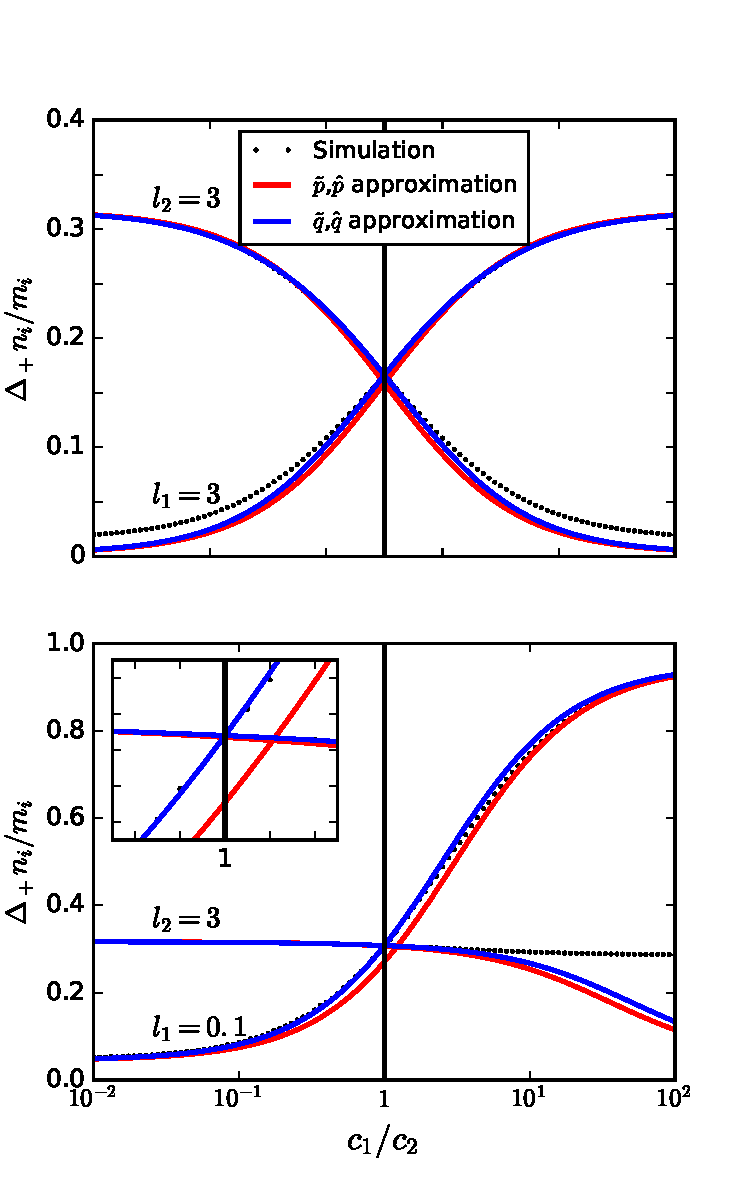
\includegraphics[scale=0.8]{approx_details.pdf}
\caption{\label{fig:approx_details} Comparison of our approximation with simulations and the naive $\tilde{p}$,$\hat{p}$ approxmation as a function of the relative $c$-advantage between two types. Our approximation breaks down in the presence of large relative $c$-advantages. The inset shows the pathology of the $\tilde{p}$,$\hat{p}$ approxmation --- in the neutral case of $c=1$ one type grows faster than the other. }
\end{figure}

Turning now to Eq.~\eqref{eq:meanfielda}, all covariances between nonfocal types are now zero, so that $\sigma_{\hat{p}}^2(\sum c_j x_j)=\sum c_j^2 \sigma_{\hat{p}}^2(x_j)$, where $\sigma_{\hat{p}}^2(x_j)=l_j$ for $j\neq i$. Here  
\begin{equation}
\sigma_{\hat{p}}^2(x_i)=\frac{l_i}{D}\left(l_i+1-e^{-l_i}-\frac{l_i}{D}\left(1-e^{-l_i}\right)^2\right),
\end{equation}
where $D= 1-(1+l_i)e^{-l_i}$, and 
\begin{equation}
\frac{\sigma_{\hat{p}}(\sum c_j x_j)}{\langle\sum c_j x_j\rangle} = \frac{\left(\sum_{j\neq i} c_j^2 l_j + c_i^2 \sigma_{\hat{p}}^2(x_i)\right)^{1/2}}{\sum_{j\neq i} c_j l_j + c_i l_i (1-e^{-l_i})/D} \label{eq:cva}.
\end{equation}

Similarly to Eq.~\eqref{eq:cvr}, the right hand side of Eq. \eqref{eq:cva} is small for both low and high nonfocal densities. Again, the worst case scenario occurs when $l_i$ and $L-l_i$ are of order $1$, but Eq.~\eqref{eq:meanfielda} is still a good approximationin this case. Again, the approxmation breaks down in the presence of a rare, strong competitor (Fig.~\ref{fig:approx_details}).

\section*{Appendix B: Total density in the Lotka-Volterra competition model}

Here we show that under the Lotka-Volterra model of competition, total density $N$ does not in general remain constant over a selective sweep in a crowded population even if the types have the same saturation density (for a related discussion on the density- and frequency-dependence of selection in the Lotka-Volterra model, see \citep{smouse_1976,mallet_2012}).

We assume equal effects of crowding within types $\alpha_{11}=\alpha_{22}=\alpha_{\rm intra}$ and $N=1/\alpha_{\rm intra}$ and check whether it is then possible for $\frac{dN}{dt}$ to be zero in the sweep ($n_1,n_2 \neq 0$). Substituting these conditions into Eq.~\eqref{eq:LV}, we obtain 
\begin{align}
\frac{d n_1}{dt} = r_1(\alpha_{11}-\alpha_{12})n_1n_2 \nonumber\\
\frac{d n_2}{dt} = r_2(\alpha_{22}-\alpha_{21})n_1n_2
\end{align}
Adding these together, $\frac{dN}{dt}$ can only be zero if 
\begin{equation}
r_1(\alpha_{\rm intra}-\alpha_{12})+r_2(\alpha_{\rm intra}-\alpha_{21})=0. \label{eq:constNcondition}
\end{equation}
To get some intuition for Eq.~\eqref{eq:constNcondition}, suppose that a mutant arises with improved competitive ability but identical intrinsic growth rate and saturation density ($r_1=r_2$ and $\alpha_{11}=\alpha_{22}$). This could represent a mutation to an interference competition trait, for example \citep{gill_1974}. Then, according the above condition, for $N$ to remain constant over the sweep, the mutant must find the wildtype more tolerable than itself by exactly the same amount that the wildtype finds the mutant less tolerable than itself. 

Even if we persuaded ourselves that this balance of inter-type interactions is plausible in some circumstances, when multiple types are present the requirement for constant $N$ becomes
\begin{equation}
\sum_{ij}r_i(\alpha_{\rm intra}-\alpha_{ij})p_ip_j=0,
\end{equation}
which depends on frequency and thus cannot be satisfied in general for constant inter-type coefficients $\alpha_{ij}$. We conclude that selection in the Lotka-Volterra competition model will generally involve non-constant $N$.

\section*{Appendix C: Density-dependence of $b$-selection}

In section ``Density-regulating traits and the threat of strong selection'' we argued that the density-dependent factor $f(\overline{b},N)$ is unchanged at the beginning and end points of an equilibrium-to-equilibrium $b$. Here we estimate the magnitude of the deviation in $f(\overline{b},N)$ during the sweep. 

For simplicity, we introduce the notation $D=N/T$ and assume that $D$ is small. We can thus make the approximation $1-e^{-\overline{b}D}\approx \overline{b}D$ and $f(\overline{b},N)\approx \overline{b}(1-D)$. We expect this to be a conservative approximate based on the worst case scenario, because $N$ is most sensitive to an increase in $b$ in this low-density linear regime. We first calculate the value of $f(\overline{b},N)$ at the halfway point in a sweep, where the halfway point is estimated with simple linear averages for $b$ and $N$. The sweep is driven by a $b$ variant with $b_j=b_i(1+\epsilon)$, and we denote the corresponding initial and final densities by $D_i$ and $D_j$ respectively, where we have $d_i=b_i(1-D_i)=b_j(1-D_j)$. We obtain
\begin{align}
f_{\rm{half}}=f(\frac{b_i+b_j}{2},\frac{N_i+N_j}{2})&=\frac{b_i+b_j}{2}\left(1-\frac{D_i+D_j}{2}\right) \nonumber \\
&=\frac{1}{4} (b_i+b_j)(2-D_i-D_j) \nonumber \\
&=\frac{1}{4} (2d_i+b_i(1-D_j)+b_j(1-N_i)).
\end{align}
Dividing by $d_i$, the proportional deviation in $f(N)$ at the midpoint of the sweep is
\begin{align}
\frac{f_{\rm{half}}}{d_i}&=\frac{1}{4}\left(2+\frac{b_i}{b_j}+\frac{b_j}{b_i}\right)\nonumber \\
&=\frac{1}{4}\left(2+\frac{1}{1+\epsilon}+1+\epsilon\right)\nonumber \\
&=1+\frac{1}{4}(\epsilon^2-\epsilon^3+\ldots),
\end{align}
where we have used the Taylor expansion $\frac{1}{1+\epsilon}=1-\epsilon+\epsilon^2-\epsilon^3+\ldots$. 

By contrast, for a $\delta$ sweep in Eq.~\eqref{eq:simplebirthdeath}, the density-dependent term $N$ increases by a factor of $\frac{1}{1-\epsilon}=1+\epsilon+\epsilon^2+\ldots$. Thus,  the deviations in $f(N)$ are an order of magnitude smaller than those shown in Fig.~\eqref{fig:strengthofselection}, and even proportional changes of order $\epsilon=0.1$ will cause a negligible deviation from the canonical selection equation.


\end{document}

